\documentclass[conference]{IEEEtran}
\usepackage[T1]{fontenc}
\usepackage{amsmath,amssymb}
\usepackage{graphicx}
\usepackage{booktabs}
\usepackage{siunitx}
\usepackage{url}
\usepackage[hidelinks]{hyperref}
\graphicspath{{../figures/}}
\sisetup{detect-all, per-mode=symbol}
\newcommand{\TBD}{\textbf{[TBD]}}

\begin{document}

\title{Drop-Foot Gait and an IMU-Triggered Ankle Exoskeleton\\in a Neuromuscular Walking Simulation}

\author{\IEEEauthorblockN{Parmida Mazloomi}
\IEEEauthorblockA{Department of Mechanical Engineering, Sharif University of Technology, Tehran, Iran}}

\maketitle

\begin{abstract}
A planar Geyer and Herr reflex walking model in SCONE was given right drop foot by weakening tibialis anterior to 50, 25 and 10\% of its strength. With its healthy controller it fell at every level below 96\%; after re-optimization of an asymmetric controller it walked at all three with a steppage gait, a plantarflexed foot and a 5 to 11\% higher cost of transport. For 25\% strength an ankle exoskeleton was built end to end: a torque requirement from the lost muscle moment, a maxon EC~45 flat motor with gear ratio 75 and a \SI{1081}{N.m/rad} series spring sized for energy per stride, a PID plus feedforward torque controller with \SI{29}{Hz} bandwidth reduced to a delay-and-lag model, and a causal heel-strike and toe-off detector on a simulated \SI{100}{Hz} shank gyroscope with noise, bias and delay. The detector found 99\% of events on simulated drop-foot gait and, unchanged, on real gyroscopes of 20 adults. A hypothesis committed before the comparison, that a phase-based active AFO restores toe clearance without lowering push-off power while the best passive AFO lowers it by more than 15\%, was rejected over three optimization seeds: the passive AFO's spring returned energy at push-off and raised the total push-off power. Neither device could be worn without re-optimizing the reflexes. After re-optimization the active AFO did not change toe clearance, which the adapted model already over-compensated, but let the model drop most of its steppage and lowered the cost of transport by 5\%.

\end{abstract}

\section{Introduction}
Drop foot is the inability to lift the forefoot, most often from weakness of tibialis anterior (TA) after peroneal nerve injury, stroke or multiple sclerosis \cite{stewart2008}. It shows in two phases of gait. In swing the toes are not lifted, so toe clearance falls and the foot can catch the ground; patients compensate with extra hip and knee flexion (steppage) or circumduction. At heel strike the missing eccentric TA moment lets the foot slap onto the floor. The clinical answer is a passive ankle-foot orthosis (AFO), a spring that holds the foot near neutral but also resists the plantarflexion needed for push-off. Active AFOs change their impedance over the cycle: braking in early stance, transparent in late stance and lifting the foot in swing \cite{blaya2004}. To do that the device must know the gait phase, and most devices estimate it from a shank-mounted inertial measurement unit (IMU).

This project asks whether such a phase-based active AFO, triggered only by a realistic simulated shank gyroscope and limited by a sized actuator, does better than the best passive AFO in a neuromuscular walking simulation of drop foot. The model is the planar Geyer and Herr reflex walker \cite{geyer2010} in SCONE \cite{geijtenbeek2019}; drop foot is a weak right TA, and the model's compensation is the re-optimization of an asymmetric reflex controller with CMA-ES \cite{hansen2016}. A similar model was used by Dermksian et al.\ \cite{dermksian} at 33\% TA strength without a device. Here the device chain is built end to end: torque requirement, motor and series elastic actuator (SEA) sizing, torque control reduced to a fitted response model, a causal gait-event detector on a sampled, noisy, biased and delayed gyroscope, and two device controllers. The hypothesis was committed to the repository before any device comparison was run, and every condition is reported over three optimization seeds, with falls counted as results.


\section{Methods}
\subsection{Model, controller and optimization}
SCONE's planar \texttt{Human0914} model (OpenSim 3 engine \cite{delp2007}) has 9 degrees of freedom, seven Hill-type muscles per leg (hamstrings, gluteus maximus, iliopsoas, vasti, gastrocnemius, soleus, TA) and compliant foot-ground contact, with a total mass of \SI{75.2}{kg}. It is driven by the Geyer and Herr reflex controller \cite{geyer2010} as implemented in the SCONE tutorials. The objective is the tutorial gait measure with the minimum speed raised to \SI{1.2}{m/s} (speeds more than 5\% below it are penalized), the Wang et al.\ metabolic cost of transport \cite{wang2012} with weight 0.1, and soft joint limits. Each evaluation simulates \SI{10}{s}; a run that ends early because the centre of mass drops is a fall. Optimizations use CMA-ES \cite{hansen2016} and are called converged when the best cost improved by less than 1\% over the last 40 generations. Every condition has three seeds (1, 2, 3); all statistics are mean and standard deviation (SD) over the seeds that walk, and falls are listed separately.

The healthy model was optimized from the tutorial result. Its stride-averaged right-leg curves (strides after the first two) are compared with the 1.2~m/s level treadmill walking of the Camargo et al.\ dataset \cite{camargo2021} (22 able-bodied adults, 568 strides) by RMSE and Pearson $r$ per curve.

\subsection{Drop-foot model and clinical metrics}
Drop foot is a scaled maximum isometric force of \texttt{tib\_ant\_r}: 50, 25 and 10\% of healthy. The \emph{immediate} effect uses the healthy controller unchanged (written once per side); the weakest strength that still walks was found by bisection. The \emph{adapted} gait re-optimizes an asymmetric controller (independent reflex parameters per leg) for 150 generations from the healthy result; seeds that had not converged by then were continued from their best parameters until they did. Metrics are computed per right stride and averaged:
minimum toe clearance (height of the \texttt{toes} origin, the metatarsophalangeal joint, over the middle half of swing; the primary metric);
ankle angle at initial contact;
peak swing dorsiflexion;
a foot-slap index, the peak plantarflexion velocity in the first 15\% of the cycle;
steppage, the change of peak swing hip and knee flexion from healthy;
peak ankle push-off power in stance;
step-length and stance-time symmetry indices \cite{robinson1987};
and the cost of transport.

\subsection{Torque requirement and actuator sizing}
The assistive torque is the TA moment that the weakness removed, $\tau_\text{req} = 1.2\,\max(0, M_\text{TA,healthy} - M_\text{TA,weak})$, from the stride-averaged moments of the healthy and adapted 25\% gaits; the 20\% is a design margin, and only dorsiflexing moments are kept because that is all TA can do. The device is a brushless DC motor (maxon EC~45 flat, \SI{70}{W}, \SI{24}{V} \cite{maxon411812}), a gear of ratio $N$ and efficiency 0.85, and a series spring $k$ \cite{pratt1995}. For a joint torque $\tau$ and angle $\theta_j$ over one stride, the gear output is $\theta_o = \theta_j + \tau/k$, the motor turns at $N\dot\theta_o$, its torque is $J_m\ddot\theta_m + b_m\dot\theta_m$ plus the reflected load, and $V = Ri + K_e\omega_m$. The design energy per stride is $\int \max(Vi, 0)\,dt$, so the drive does not regenerate (copper losses are inside $Vi$). A design is feasible if peak speed, RMS current (rated \SI{3.21}{A}), peak current (\SI{15}{A}, the drive) and peak voltage stay within limits. The sweep covers $N = 20$ to 150 and 25 stiffnesses from 50 to \SI{2000}{N.m/rad} plus the rigid case. The chosen design is the most compliant one within 2\% of the lowest feasible energy.

The joint trajectory in this calculation is the normative ankle angle \cite{camargo2021} resampled to the model's stride time, not the model's own. The adapted model's ankle slaps down after heel strike (Section~\ref{sec:res-healthy}), reaching \SI{15}{rad/s} and \SI{2100}{rad/s^2}; the reflected rotor inertia then needs more RMS current than the motor's rating for every $N$ and $k$, while the human trajectory peaks at \SI{4}{rad/s} and \SI{66}{rad/s^2}. Both sweeps are reported. Gait curves on the 1\% grid are resampled with periodic cubic splines, because linear interpolation turns the second derivative into impulses at the grid points.

\subsection{Simulated shank gyroscope and event detector}
A Lua script controller reads the sagittal angular velocity of \texttt{tibia\_r} every control step and turns it into a gyroscope signal: samples at \SI{100}{Hz}, white noise of \SI{0.5}{\degree/s} RMS, a bias of \SI{2}{\degree/s}, a \SI{15}{ms} transport delay and a zero-order hold. The causal detector uses the classic shank pattern \cite{aminian2002}: it arms on the positive mid-swing peak, takes heel strike (HS) as the first negative minimum after the terminal-swing zero crossing (feature \emph{min}) or the zero crossing itself (\emph{zero}), and toe-off (TO) as the next negative minimum after a lockout of part of the mean stride. Gait phase is the time since HS divided by the mean of the last three stride times. Each Lua module has a Python twin that reproduces it to rounding error on the same samples, and the noise generator is shared bit for bit. Ground truth is the right vertical ground reaction force crossing 5\% of body weight. Errors are estimate minus truth, latency is confirmation time minus truth, and an estimate pairs with a true event if it falls within $-150$ to $+250$~ms. The detector was validated on three 60~s healthy runs and on the adapted 25\% gait, and then, unchanged, on the shank gyroscopes of the Camargo et al.\ subjects at 1.2~m/s.

\subsection{SEA torque control}
For the chosen $N$ and $k$, the plant is the reflected rotor inertia $J_r = J_m N^2$ and damping $b_r = b_m N^2$ driven by $\eta N K_t i$, the spring torque $\tau = k(\theta_o - \theta_j)$, and the motor winding with a \SI{1}{kHz} PI current loop that saturates at the supply voltage and the drive's peak current. The torque controller runs at \SI{1}{kHz} with one sample of computation delay:
\begin{equation}
u = u_\text{ff} + K_p e + K_i\!\int\! e\,dt - K_d \dot\tau_f,\quad i_\text{cmd} = u / (\eta N K_t),
\end{equation}
with $e = \tau_d - \tau$, the derivative on the measured torque filtered at \SI{100}{Hz}, and anti-windup. The feedforward is the static term $\tau_d$ plus a model term $J_r(\ddot\theta_j + \ddot\tau_d/k) + b_r(\dot\theta_j + \dot\tau_d/k) + K_d\dot\tau_{d,f}$ \cite{vallery2007,paine2014}. The last term matters: without it the derivative on measurement still acts when tracking is perfect, and at the lightly damped locked-output resonance it dominates and opens a 15~dB notch in the closed-loop response. Gains place the locked-output poles at a natural frequency $\omega_n$ with damping 0.7 and the integral zero a factor of five below. The design is the lowest $\omega_n/2\pi$ on a 5~Hz grid, above the locked resonance, whose small-signal response has less than 6~dB of peaking, a bandwidth of at least 10~Hz without the model feedforward, and an RMS error under 10\% of peak on five strides of $\tau_\text{req}$ with saturation. Bode plots come from simulated sine responses with the output locked. The closed loop is then reduced to a pure delay plus a first-order lag, fitted by grid search to the tracking response.

\subsection{Devices and controllers in SCONE}
The device is a moment pair, $+\tau$ on \texttt{talus\_r} and $-\tau$ on \texttt{tibia\_r} (positive dorsiflexes). SCONE external moments persist, so the script adds only the change of moment at each step; a constant-torque pulse test confirmed the bookkeeping. The \emph{passive AFO} is $\tau = -k_\text{AFO}\theta$ with neutral angle 0. The \emph{active AFO} is a finite-state machine driven only by the detector: from HS to 15\% of the estimated cycle, viscous braking $\tau = \max(0, -b\dot\theta)$ with $b = \SI{1}{N.m.s/rad}$; then zero torque until TO; in swing, PD control toward a dorsiflexed target, $\tau = \max(0, k_p(\theta^* - \theta) - k_d\dot\theta)$ with $k_p = \SI{30}{N.m/rad}$ and $k_d = \SI{0.6}{N.m.s/rad}$, until the next HS or a 0.8~s timeout. The gains come from a sizing calculation against the healthy TA moments, not from tuning. The command passes through the fitted actuator model and is clipped at the peak of $\tau_\text{req}$. The device never plantarflexes.

\subsection{Experiment}
Conditions: healthy; drop foot at 25\% TA strength with no device; with the passive AFO; with the active AFO. Each device condition is run with the adapted drop-foot controller \emph{frozen} (the first day with the device) and \emph{re-optimized} for 150 more generations with the device on, from the adapted controller of the same seed (adaptation). Because re-optimization adds generations, the no-device condition is re-optimized for the same 150 generations as a control. The passive stiffness ($k_\text{AFO} = 10$ to \SI{160}{N.m/rad}, factors of two) and the active swing target ($\theta^* = 0$, 5, \SI{10}{\degree}) were each chosen on the frozen controllers by one rule: among the settings with which all seeds walk, the one with toe clearance closest to healthy, the lower setting on a tie. A trial of the pipeline showed that no setting may let all seeds walk, so before the comparison the rule was completed for both devices: among the settings with the most seeds walking, the toe clearance closest to healthy decides, and if no seed walks at all, the longest mean time before the fall.

The hypothesis, committed before any comparison: \emph{at 25\% TA strength, after re-optimization with the device, the active AFO brings mid-swing toe clearance to within 10~mm of healthy without lowering peak ankle push-off power (muscles plus device) by more than 10\% compared with no device, while the best passive AFO lowers it by more than 15\%.} Each of the three parts holds or fails on the seed means; a part that misses by less than one seed SD is inconclusive, and a fall in any seed fails the active parts.

Robustness of the re-optimized conditions was tested at a second speed (all conditions re-optimized with a 1.5~m/s minimum), with the gyroscope noise and delay doubled, with IMU and actuator delays from 0 to 100~ms, and with single \SI{0.2}{s} horizontal pushes on the pelvis as in the SCONE perturbation tutorial, from 25 to 150~N in both directions.


\section{Results}
\subsection{Healthy baseline}\label{sec:res-healthy}
The three healthy seeds converged to nearly the same gait (costs 0.5447 to 0.5467, Fig.~\ref{fig:healthy}): \SI{1.16}{m/s}, stride \SI{1.36}{s} and \SI{1.57}{m}, stance 61.7\% of the cycle against $60.3 \pm 1.0\%$ in the data, and a cost of transport of \SI{5.46}{J/(kg.m)}. Shapes agree well ($r = 0.95$ to 0.97 for hip and knee angles, ankle moment and vertical force, 0.96 for the shank angular velocity that the detector uses, 0.83 for the ankle angle). The largest error is a constant hip offset of \SI{+19}{\degree} (RMSE \SI{7}{\degree} without it): the model walks with its pelvis tilted forward by \SI{13}{\degree}. The stance knee extends fully in mid stance, and the ankle drops from 0 to \SI{-20}{\degree} within 3\% of the cycle after heel strike (peak plantarflexion velocity \SI{780}{\degree/s}, impact peak 1.55 body weights): the optimized healthy model already has little eccentric control of the foot at loading. Foot slap in drop foot is therefore judged against this model value. Mid-swing toe clearance is \SI{36}{mm}.

\begin{figure}[t]
\centering
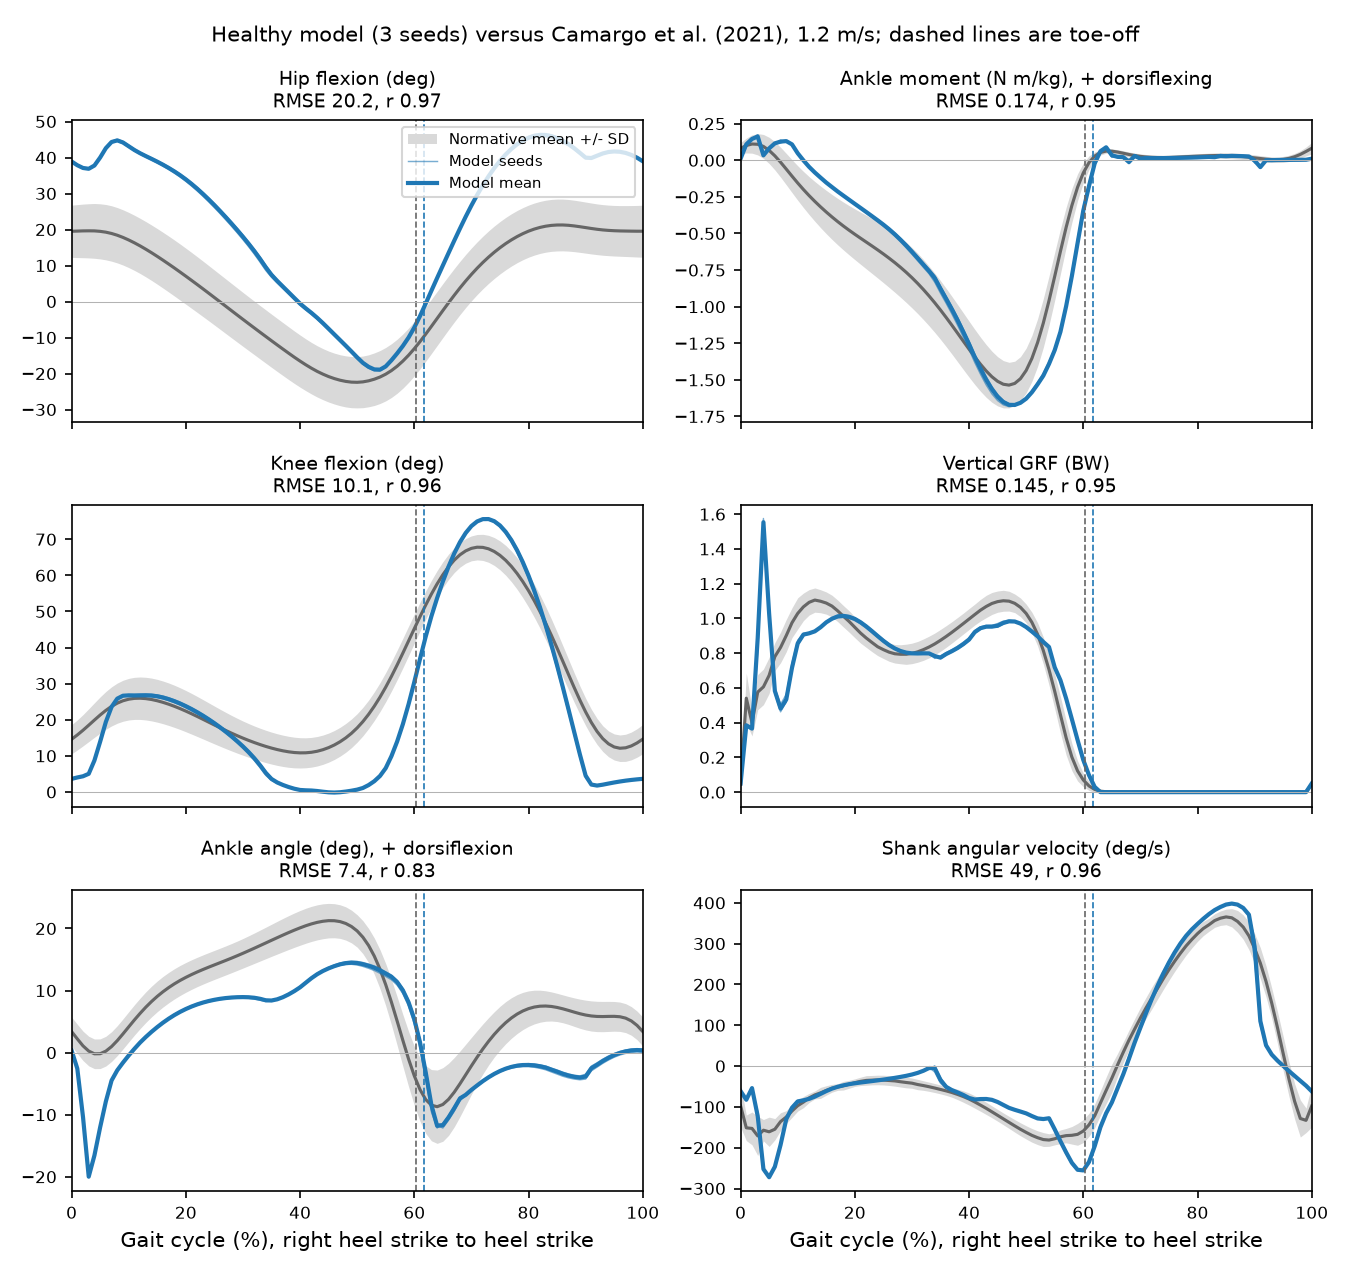
\includegraphics[width=\columnwidth]{healthy_vs_normative.png}
\caption{Healthy model (three seeds) against the Camargo et al.\ \cite{camargo2021} mean and SD at 1.2~m/s, right stride.}
\label{fig:healthy}
\end{figure}

\subsection{Drop foot}
\emph{Immediate effect.} With the healthy controller unchanged, the model falls at every strength from 10 to 90\%, in all three seeds, within 1.3 to 1.6~s below 90\%. It trips: at 50\% the right foot touches the ground 0.20~s after toe-off. The weakest strength that still walks 10~s is 96.3 to 98.8\% depending on the seed. The healthy gait is an effort optimum with no reserve (peak swing TA activation 0.15), so no immediate-effect gait metrics exist.

\emph{Adapted gait.} After re-optimization all three seeds walk at every strength (Table~\ref{tab:dropfoot}, Fig.~\ref{fig:dropfoot}). The 10\% seeds needed the longest search: after 150 generations only one walked, and after 300 to 410 all three did, with costs (0.563 to 0.589) as low as at 25\% (0.590 to 0.695). One seed at 50\% ended 1.3\% better over its last 40 generations, just above the convergence criterion. The adapted model shows the clinical picture of drop foot: the ankle hangs 15 to \SI{30}{\degree} plantarflexed in mid swing and lands plantarflexed, and the leg is lifted more, mainly at the hip (steppage of +6 to \SI{+11}{\degree}) and less at the knee (+3 to \SI{+4}{\degree}). The weak TA is activated more (swing peaks of about 0.2, 0.45 and 0.6 against 0.15). The compensation overshoots: mid-swing toe clearance is 9 to 20~mm \emph{above} healthy. The cost of transport rises by 5 to 11\%, push-off power is unchanged within the seed spread, and foot slap rises only by 5 to 11\% because the healthy model already slaps. The CMU 2D model at 33\% strength \cite{dermksian} walked at \SI{0.65}{m/s} with an exaggerated knee lift; here the stride is longer and faster (\SI{1.77}{m} in \SI{1.38}{s} at 25\%) because the objective penalizes walking below \SI{1.2}{m/s}, and the extra lift is mostly at the hip.

\begin{table}[t]
\centering
\caption{Right-side metrics of the adapted gaits, mean $\pm$ SD over three seeds (all walk).}
\label{tab:dropfoot}
\footnotesize
\setlength{\tabcolsep}{3pt}
\begin{tabular}{lcccc}
\toprule
Metric & Healthy & 50\% & 25\% & 10\% \\
\midrule
Toe clearance (mm) & $36.3 \pm 0.3$ & $45.5 \pm 1.5$ & $56.5 \pm 4.9$ & $49.9 \pm 8.9$ \\
Ankle at IC (\si{\degree}) & $0.4 \pm 0.3$ & $-2.8 \pm 5.0$ & $-6.8 \pm 2.5$ & $-8.7 \pm 4.9$ \\
Swing dorsiflexion (\si{\degree}) & $0.4 \pm 0.3$ & $-2.8 \pm 5.0$ & $-6.7 \pm 2.5$ & $-5.7 \pm 6.5$ \\
Foot slap (\si{\degree/s}) & $782 \pm 5$ & $871 \pm 71$ & $824 \pm 31$ & $844 \pm 117$ \\
Steppage, hip (\si{\degree}) & 0 & $+6.0 \pm 2.7$ & $+10.9 \pm 0.9$ & $+9.7 \pm 1.4$ \\
Steppage, knee (\si{\degree}) & 0 & $+3.0 \pm 1.7$ & $+4.1 \pm 1.6$ & $+2.9 \pm 2.6$ \\
Push-off power (W) & $126 \pm 1$ & $132 \pm 2$ & $124 \pm 4$ & $122 \pm 9$ \\
Speed (m/s) & $1.16$ & $1.23$ & $1.28$ & $1.20$ \\
CoT (J/(kg\,m)) & $5.46$ & $5.87$ & $6.05$ & $5.71$ \\
\bottomrule
\end{tabular}
\end{table}

\begin{figure}[t]
\centering
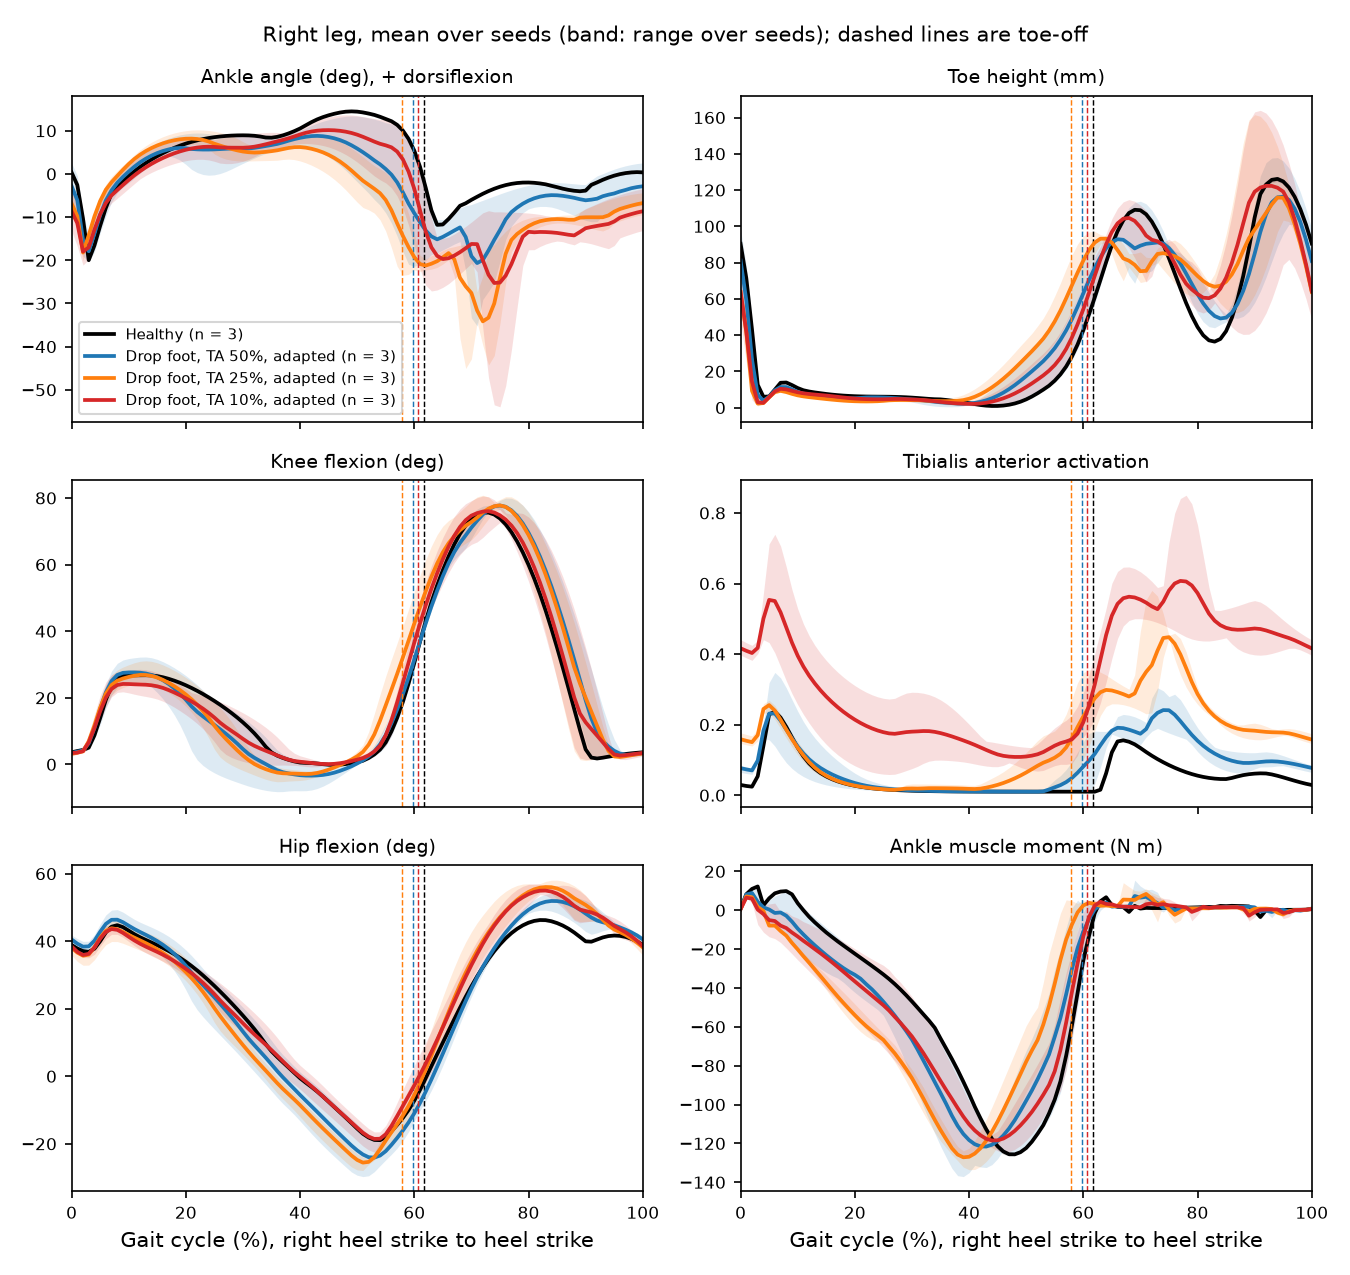
\includegraphics[width=\columnwidth]{dropfoot_overlay.png}
\caption{Right-leg curves of the healthy and adapted drop-foot gaits, mean over seeds with the range as a band; dashed lines mark toe-off.}
\label{fig:dropfoot}
\end{figure}

\subsection{Actuator sizing}
The TA deficit at 25\% strength has two parts (Fig.~\ref{fig:actuator}a): braking the foot after heel strike, with the peak requirement of \SI{13.6}{N.m} at 8\% of the cycle, and lifting it in swing, up to about \SI{7}{N.m}. On the normative trajectory 250 of the 702 designs are feasible (Fig.~\ref{fig:actuator}b). The chosen design is $N = 75$ with $k = \SI{1081}{N.m/rad}$: \SI{6.76}{J} per stride (\SI{6.03}{J} with ideal regeneration), RMS current \SI{1.79}{A}, peak motor speed \SI{301}{rad/s} and peak voltage \SI{11.3}{V}. A rigid drive at the same ratio needs \SI{6.79}{J}, so the spring saves 0.4\%. Series elasticity saves motor work when the spring stores and returns a large share of the joint work, as in push-off assistance \cite{au2008}; a dorsiflexion assist has small torques at large ankle velocities, the spring deflects by a fraction of a degree, and the copper losses depend on torque, not stiffness. The spring is kept for torque sensing and impact tolerance. On the model's own ankle trajectory no design is feasible (lowest RMS current \SI{3.64}{A} against the \SI{3.21}{A} rating), because of the foot slap.

\begin{figure}[t]
\centering
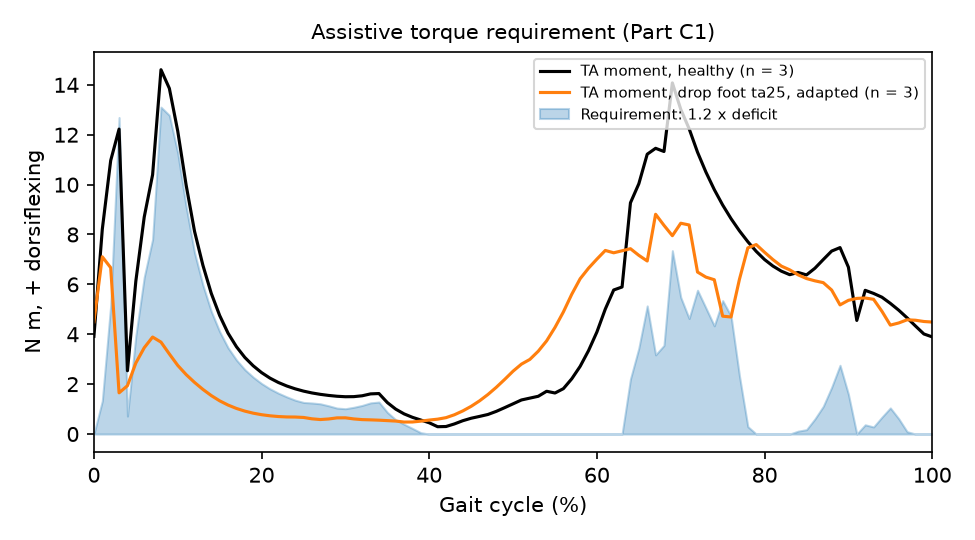
\includegraphics[width=\columnwidth]{actuator_requirement.png}\\[2pt]
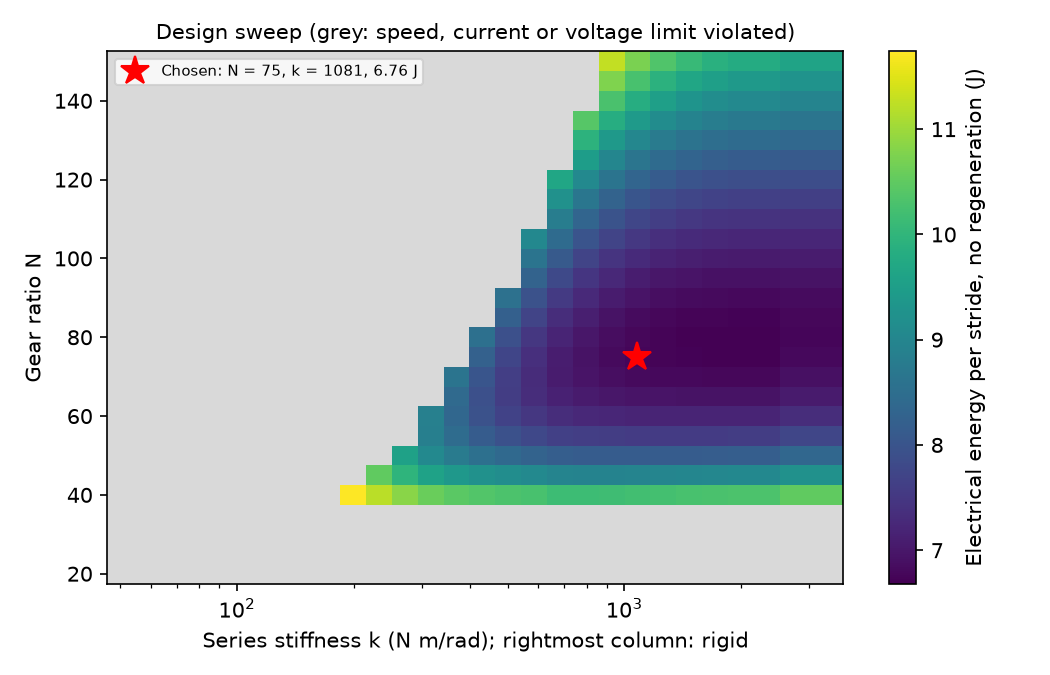
\includegraphics[width=\columnwidth]{actuator_sweep.png}
\caption{(a) TA moment of the healthy and adapted 25\% gaits (three seeds each) and the requirement, 1.2 times the deficit. (b) Electrical energy per stride over gear ratio and series stiffness on the normative ankle trajectory; grey designs exceed a speed, current or voltage limit.}
\label{fig:actuator}
\end{figure}

\subsection{Gait-event detection}
On 127 healthy heel strikes and 129 toe-offs (three 60~s runs) both HS features found every event with no false detection. The \emph{min} feature estimates HS $25.4 \pm 2.9$~ms late, confirmed 37.8~ms after the event; \emph{zero} fires $50.6 \pm 1.4$~ms early, before the foot lands. TO is estimated $13.0 \pm 3.0$~ms early. The rule fixed before the results (no missed or false events, then the lower HS mean absolute error) selected \emph{min}; the gait-phase error is $-1.5\%$ mean, 2.4\% RMS of the cycle. The Lua detector and its Python twin agree to $10^{-14}$~s. On the adapted 25\% gait (112 HS and 114 TO; seed 3 falls after 41.5~s of the 60~s run) the detector still found 99\% of the events, with one missed HS and two missed TO, all in one seed. The errors widen: HS with \emph{min} $+23.7 \pm 14.1$~ms and TO $-26.8 \pm 22.0$~ms, phase error 2.8\% RMS. The \emph{zero} feature fails on drop foot, firing 39 to 119~ms early depending on the seed, because the adapted gaits differ in how long the shank keeps swinging before the flat-footed contact. The choice of \emph{min} stands.

Without retuning, on the real shank gyroscopes of 20 Camargo subjects (two rejected because the gyroscope could not be aligned with motion capture), the detector found 535 of 536 heel strikes and 527 of 532 toe-offs, with one false detection each. The HS error with \emph{min} is bimodal, $+12.4 \pm 20.6$~ms: near zero in most subjects, but about $+50$~ms in the two subjects whose gyroscope axis has the opposite sign to the other eighteen (probably mounted differently), where the shallow contact notch is missing and the detector waits for the impact minimum. TO is estimated earlier and with more spread than in simulation ($-40.8 \pm 26.1$~ms). Between-subject variation, absent in a single model, is the main source of error on real data.

\subsection{SEA torque control}
The locked-output resonance of the chosen SEA is at \SI{16.4}{Hz}. Designs from 20 to \SI{30}{Hz} are stable with little peaking; 35 and \SI{40}{Hz} have more than 6~dB of peaking and from \SI{45}{Hz} the sampled loop is unstable. The selected \SI{20}{Hz} design ($K_p = 0.487$, $K_i = 37.4$, $K_d = 0.0165$, in A per N\,m units) has a \SI{-3}{dB} bandwidth of \SI{28.8}{Hz} with static feedforward and \SI{134}{Hz} with the model feedforward (Fig.~\ref{fig:sea}). At the full \SI{13.6}{N.m} amplitude the current and voltage limits change no gain by more than 1~dB up to \SI{200}{Hz}. It tracks five strides of $\tau_\text{req}$ with an RMS error of \SI{0.21}{N.m} (1.5\% of peak; \SI{1.87}{N.m} without the model feedforward), a peak current of \SI{11.4}{A} and no clipping. Fitted to the loop with static feedforward, the reduced model is an 8~ms delay and a 3.3~ms lag (RMS misfit \SI{1.16}{N.m}); with the model feedforward it is a 1~ms delay and no lag. The simulated device uses the former, which does not assume that the ankle trajectory is known ahead of time.

\begin{figure}[t]
\centering
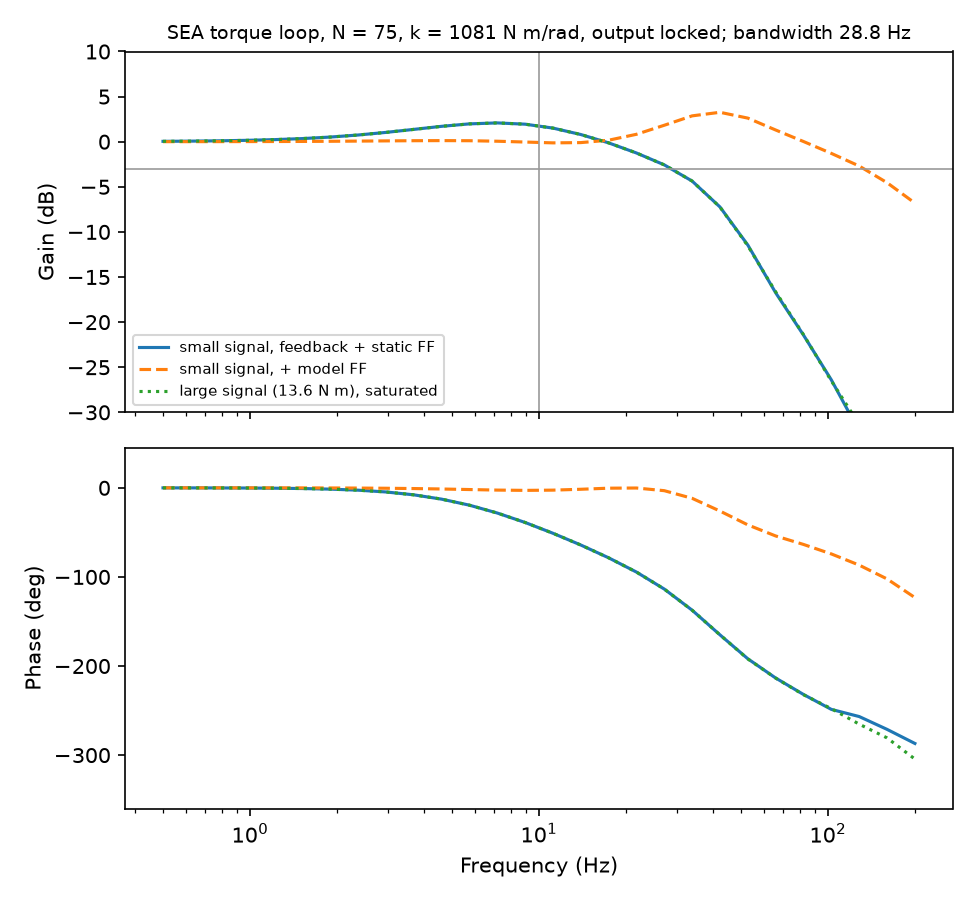
\includegraphics[width=\columnwidth]{sea_bode.png}
\caption{Closed-loop torque response of the SEA with the output locked: feedback with static feedforward, with the model feedforward, and at the full torque amplitude with current and voltage saturation.}
\label{fig:sea}
\end{figure}

\subsection{Device experiment}
\TBD

\subsection{Robustness}
\TBD


\section{Discussion}
\emph{The hypothesis failed on the passive AFO, for a reason the hypothesis did not anticipate.} A passive AFO is expected to cost push-off because it resists plantarflexion. With its neutral angle at 0 and a stiffness of \SI{160}{N.m/rad}, the spring chosen by the rule instead stores energy in the stance dorsiflexion and returns it in early push-off, so the total ankle power rises while the muscles' share falls by 9\%. Whether a passive AFO costs push-off depends on its neutral angle and on how far the ankle dorsiflexes before push-off, not only on its stiffness. A clinical posterior leaf-spring AFO is set near neutral too, but the model's stance dorsiflexion of up to \SI{10}{\degree} under a stiff spring is more than an orthosis with soft-tissue compliance would see. The result is a statement about this metric and this spring, not evidence that passive AFOs help push-off.

\emph{Toe clearance was the wrong primary metric for an adapted model.} The adapted model already cleared its toe 9 to 20~mm \emph{higher} than healthy by lifting the hip, so part 1 could only fail if a device made clearance worse. It did not discriminate between the devices: all three re-optimized conditions have the same mean clearance. What the active AFO changed was how the clearance was produced: with the foot held up, the re-optimized controller gave up most of the steppage, and the cost of transport fell by 5\%, about two thirds of the way back to healthy. Steppage or the cost of transport would have been the more telling primary metric, and the toe clearance threshold should have been two-sided. Both choices are recorded here as lessons, not applied after the fact.

\emph{Adaptation dominates.} No device setting could be worn by the frozen controllers, and even a \SI{5}{N.m/rad} spring made them fall. The comparison between devices is therefore only meaningful after re-optimization, which assumes the wearer re-tunes the whole gait to the device. People adapt partly and over time; the truth for a first session lies between a model that falls and a model that has fully re-optimized. Device studies on optimized reflex models should report both, as here, and should not read the frozen results as a prediction of a person's first steps.

\emph{The sensing and actuation chain was not the bottleneck.} The shank-gyroscope detector found 99\% of the events on drop-foot gait with heel-strike errors of about 24~ms, and transferred to real gyroscopes without retuning. Doubling its noise changed nothing. The SEA tracked the requirement to 1.5\% with no saturation, and the simulated device used the slower fitted response without the model feedforward. The fragility of the re-optimized gaits to timing (one seed falls at any IMU or actuator delay other than the nominal one) comes from the optimized gait, not from the device: the active AFO itself still lifted the foot at 100~ms of delay. For the drop-foot deficit the series spring saved almost no energy; its value in such a device is torque sensing and impact tolerance.


\section{Limitations}
\emph{Planar model.} \texttt{Human0914} moves in the sagittal plane only, with seven muscles per leg, no subtalar or metatarsophalangeal joint and no arms. Patients with drop foot often clear the foot by hip circumduction or hip hiking; the model cannot, so it shows only the sagittal compensations (steppage and changed timing), which exaggerates them, as Dermksian et al.\ also noted \cite{dermksian}. Without a toe joint, toe clearance is the height of a point fixed to the foot.

\emph{A reflex controller is not a patient.} Drop foot here is a weaker TA with intact sensing and reflexes; a peroneal nerve lesion or a stroke also changes sensation, spasticity and the other muscles. ``Adaptation'' is a re-optimization of reflex parameters for effort and speed, run to convergence. A person adapts for other goals (stability, fear of falling, comfort), partly within a session, and does not reach an optimum. The frozen and re-optimized conditions bracket the first day and a fully adapted user; neither is a clinical prediction. The optimized gaits also have little reserve: the healthy controller falls with a 2~N\,m pulse in swing, and the adapted gaits fall after modest pushes, which is not how people walk.

\emph{Idealized attachment.} The device applies an exact moment pair to the shank and the foot. There is no strap or cuff compliance, no misalignment between the device and the anatomical joint, no added mass or inertia, and no friction. Real orthoses lose part of their torque to soft tissue and shift during use; the added distal mass alone would raise the swing cost.

\emph{Optimizer randomness.} CMA-ES finds different local optima from different seeds: the 50\% runs differ in cost by 40\% between seeds. Three seeds show this spread but do not measure it well, and an SD over three values is a weak basis for the inconclusive band of the decision rule. Each run was stopped at a fixed number of generations, and convergence was checked on the cost history only.

\emph{Device chain.} The actuator was sized and its controller designed offline, against the normative ankle trajectory rather than the model's own, and the SCONE device sees only the fitted delay and lag, not the full SEA dynamics, motor heating or the drive. The detector was tuned on simulated gait of a model whose strides are nearly identical; the real-data test shows larger, subject-dependent errors. The active controller's gains came from a sizing calculation and only the swing target was chosen, by a rule fixed in advance; other gains would give other results.

\emph{Measures.} Ten-second simulations give four analysed strides per run. The metabolic cost is the Wang et al.\ model \cite{wang2012} inside the objective, not a measured quantity, and the device's electrical energy is reported separately and not added to it.


\section*{Reproducibility}
Code, scenarios, the optimized controller parameters and every table are in the project repository; each figure is regenerated by \texttt{python analysis/make\_figures.py}. The Camargo et al.\ data are used under CC BY 4.0 and are not redistributed.

\bibliographystyle{IEEEtran}
\bibliography{refs}

\end{document}
